%!TEX root = thesis.tex

\chapter{Thematic.js - a Reusable Visualization Tool}
\label{chapter:implementation}

% 10-15 pages?

% You have now explained how you are going to tackle your problem. 
% Go do that now! Come back when the problem is solved!

% Now, how did you solve the problem? 
% Explain how you implemented your solution, be it a software component, a
% custom-made FPGA, a fried jelly bean, or whatever.
% Describe the problems you encountered with your implementation work.

As discussed in the chapter \ref{chapter:reuse}, reusing software typically leads to increased productivity and better quality. Therefore, to achieve the targets of this thesis, we decided to implement a reusable visualization tool. As the tool is designed to benefit building geographical visualizations, or thematic maps, on the web, we decided to name the tool Thematic.js.

\section{Problem Setting}

Currently, when building a visualization for geographical data, it is unnecessarily laborious to develop the visualization from the beginning using low abstraction level APIs provided by mapping libraries. Consequently, when visualizing data suitable to be visualized with more complicated visualization methods such as isarithmic maps, it is not feasible to use the most suitable visualization methods. \emph{This encourages the visualizer to use a simpler, yet less suitable method such as a dot map.}

Second, when building web-based geographical visualizations, it is typically needed to build the whole visualization architecture using web technology such as HTML\footnote{\url{http://www.w3.org/TR/html5/}} and ECMAScript\footnote{\url{http://www.ecma-international.org/ecma-262/5.1/}}. Therefore, an astonishing amount of knowledge of such technology is required to even develop a simple map visualization. \fixme{Do these require some concrete or literature proof?}

\section{Application Requirements and Design}
\label{section:requirements}

We started the implementation process by analyzing the requirements of the different geographic visualization methods presented in chapter \ref{subsection:mappingmethods}. Specifically, we analyzed the underlying structure of the visualizations in order to abstract the applicable parts as reusable components. For this, we adopted the ``hot spot'' method by \citet{schmid_systematic_1997} for detecting similarities and dissimilarities in software.

\emph{In order to solve both problems presented in the previous section, we decided to implement a dual approach for visualization.} As one of the problems related to visualizations is the amount of application architecture work needed, the tool should provide a so-called whole-page scaffold architecture \citep{jazayeri_trends_2007} which contains the needed page-specific architecture. We call this part of the system \emph{framework}. However, as the framework approach involves challenges regarding integrations, we decided to also implement an independent visualization component in order to support integration of the visualization in existing web pages. We call this part \emph{library}. When referring to both of the parts of the system, we use the term \emph{application}.

\subsection{Reuse Methods}

We gathered the analyzed data about the requirements in addition to problems discussed in the previous chapter, and determined the forms of reuse applicable in this case. Since the techniques are not mutually exclusive and each has its own benefits, we decided to use a combination of multiple techniques. 

The application was developed, and can be used with, the JavaScript language, which is a relatively high-level programming language. The scaffold architecture uses the framework method for enabling the visualizer to get started with the visualization quickly while allowing thorough customization later if needed. The visualization library is built as a collection of software components, which allow versatile functionality and composability while abstracting the implementation details. Moreover, the tool contains example visualizations which can be used as a starting point for building visualizations using the design and code scavenging method.

\subsection{Supported visualization methods}
\label{subsection:supportedvisualizationmethods}

As discussed in the chapter \ref{subsection:mappingmethods}, several different thematic mapping methods exist. As some of these methods are fundamentally different in implementation, it was needed to explicitly consider the requirements of each method. It was also necessary to decide whether to implement support for each method, as support for some of the methods might have been needed to be dropped in order to manage the application complexity and the scope of this work. In order to support the most frequent use cases, we decided to implement support for the following visualization methods:

\begin{itemize}
	\item Choropleth maps
	\item Dasymetric maps
	\item Isarithmic maps
	\item Dot maps
	\item Proportional Symbol maps
\end{itemize}

Of the visualization methods presented in section \ref{subsection:mappingmethods}, we decided to exclude explicit multivariate maps, cartograms and flow maps. The decision was made primarily due to the fact that of the methods presented, these are the least frequently used. Moreover, since there are several fundamentally different design options for some of the methods, such as multivariate maps, it is considerably more difficult to abstract the implementation details to provide a general-purpose visualization module. However, it should be noted that the modular architecture of the application enables easy extendability to support these types of visualizations in the future. Additionally, multivariate maps can be achieved to some degree by using several of the implemented map methods simultaneously.

\section{Application Architecture}

In the highest level, the application architecture consists of two parts: the visualization framework and the visualization library. While the framework uses the library for visualization, it also consists of other functionality and the library can be used separately of the framework. The architecture of the framework is presented in figure \ref{fig:framework_architecture}.

Framework consists of a Single-Page Web Application (SPA) which embeds the visualization library along with other functionality necessary or beneficial for user experience. Notably, the application uses HTML and CSS for displaying the page correctly and HTML5 Application Cache\footnote{\url{http://www.w3.org/TR/html5/browsers.html}} for offline availability and faster loading times. Application also contains functionality for displaying the visualization correctly on devices of different sizes and capabilities.

\begin{figure}[htbp]
  \centering
  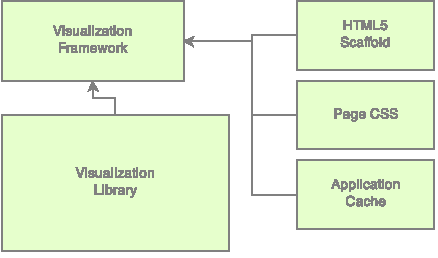
\includegraphics[width=\textwidth]{images/framework-architecture.pdf}
  \caption{The architecture of the Thematic.js framework.}
  \label{fig:framework_architecture}
\end{figure}

\begin{figure}[htbp]
  \centering
  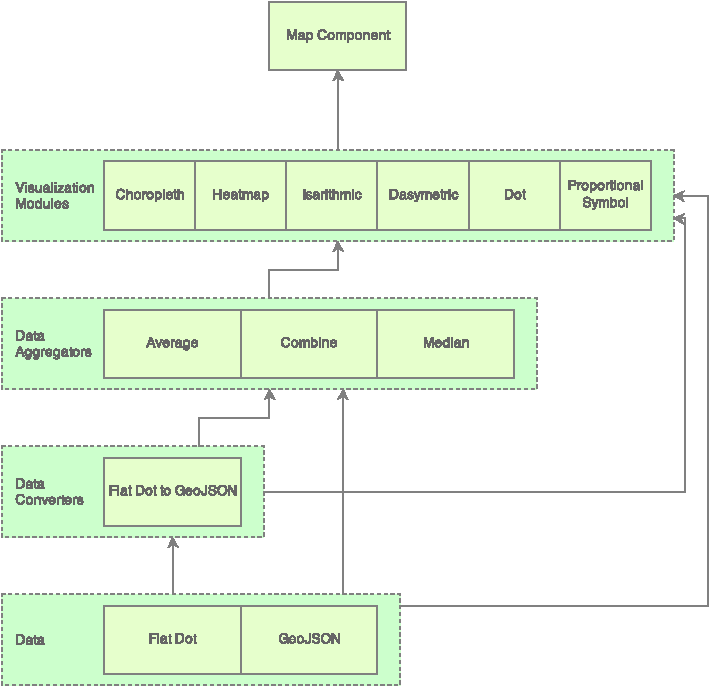
\includegraphics[width=\textwidth]{images/library-architecture.pdf}
  \caption{The architecture of the Thematic.js library. Arrows denote the flow of data.}
  \label{fig:lib_architecture}
\end{figure}

The architecture of the library is described in figure \ref{fig:lib_architecture}. The library consists of a map component, mapping modules, data aggregators and data converters. The map component is used for displaying the map layer and for managing mapping modules. The component can be added to any block-level element on a web page. Internally, the map is displayed using Leaflet\footnote{\url{http://leafletjs.com/}}. 

Individual mapping modules are added to the map as Leaflet layers. For convenience and maintainability, we created an abstract mapping module for handling system-specific procedures such as keeping module status. The abstract module should be used as an object prototype for all mapping modules. Individual mapping modules each support a mapping method, but all can be customized to a degree. Currently, the modules only support GeoJSON\footnote{Geographic JavaScript Object Notation, \url{http://www.geojson.org}} data, but there are no technical restrictions on using any format of data.

Typically, mapping modules are used with some external data. The data is often in a non-standard format as presented in section \ref{section:evaluatedcases}. For this, data converters are used. Data converters are straightforward stateless components which transform data from a non-standard format to format supported by the mapping modules. For example, the library provides a converter from ``flat dot'' JSON format (see appendix \ref{appendix:flatdotformat}) to standard GeoJSON FeatureCollections.

Aggregators are similar to converters in the sense that both transform data. However, while converters do 1-to-1 conversions, aggregators combine several grouped data sets into one by, e.g., calculating an average of the values in sets.
	
The use of converters and aggregators is not required when creating a visualization if the data is in the correct format, but the components help bring a structured way of transforming the data into appropriate format.

\section{Supported Platforms}

The application is developed using standard web technology. Theoretically, this means that the app supports all HTML5, CSS3 and ECMAScript 6 compliant browsers. However, in practice, none of the widely used browsers support the standards completely \citep{manian_html5_2011}. Therefore, we have tested the application on some the most widely used modern web browsers, i.e., the latest versions of Google Chrome (38), Mozilla Firefox (33), Apple Safari (8), Opera (25), Microsoft Internet Explorer (11)\footnote{Internet Explorer 11 requires additional ES6 Promises polyfill, \url{https://github.com/jakearchibald/es6-promise}}, Apple iOS Safari (8) and Google Android Chrome (38). In total, this represents the browsers of 66 \% of Internet users \citep{statcounter_globalstats_2014}. \fixme{Verify the support with Android Chrome}.

While the application is most naturally run in a web environment, it is also possible to embed the system to various native applications using a web view component. Web view components are available on at least Windows \citep{small_ten_2012}, Mac OS X \citep{hunter_why_2014}, Android \citep{google_building_2014} and iOS \citep{apple_uiwebview_2014} platforms.

Due to the dual approach described in chapter \ref{section:requirements}, the application can be used in almost any existing web application, using almost any framework and library. However, due to a possibility of a namespace collision, other libraries using global namespaces \texttt{L} (Leaflet), \texttt{\char`_} (underscore), or \texttt{thematic} may cause an incompatibility with the application as described in \citet{osmani_essential_2011}.

\section{Implemented Functionality}

The following sections present the most important application functionality, namely supported mapping methods, managing input formats and values, and modularity for supporting future extensions.

\subsection{Choropleth Maps}

Choropleth maps are used for visualizing enumerated or areally aggregated data \citep[chap.~6]{dent_cartography:_2008}. According to \citet[chap.~14]{slocum_thematic_2014}, it is the most frequently used mapping method. Therefore, implementing choropleth mapping functionality is essential for a successful mapping tool.

To use choropleth mapping, visualizer uses the choropleth mapping module of the application. If the user already has the relevant data in GeoJSON format, nothing else is required. However, if the relevant data is stored separately of the designated area definitions, the user needs to use the \emph{combine} aggregator provided by the application. The aggregator associates the data with the area definition in question and outputs the data in GeoJSON format supported by the mapping module. An example code for using the choropleth module is presented in listing \ref{listing:choropleth}.

\begin{lstlisting}[caption=Using the choropleth mapping module with Thematic.js.,language=JavaScript,label=listing:choropleth]
var Choropleth = thematic.modules.Choropleth;
map.addModule('voting', new Choropleth({field: 'value'})
    .setScale(scaleFn)
    .setData(data));
\end{lstlisting}

\subsection{Dasymetric Maps}

Dasymetric maps are supported in an approximated fashion: the dasymetric mapping module approximates dasymetric data by using the floating grid method as presented by \citet{langford_generating_1994}. The module is provided the grid of dots in GeoJSON format as data, and the data is used to generate appropriate dasymetric map approximation. The data can also be aggregated and converted using any of the supplied aggregators and converters.

\subsection{Isarithmic Maps}

The application provides two isarithmic mapping modules: the Isarithmic module enables approximated isarithmic mapping while the Heatmap module enables heat map visualizations. Heatmap method is more accurate than the approximated isarithmic method, but requires a dot-like data set in order to provide best results. The approximated isarithmic module employs the floating grid method of \citet{langford_generating_1994}. An example isarithmic visualization built with Thematic.js is presented in figure \ref{fig:isarithmicimpl}.

\begin{figure}[htbp]
  \begin{center}
    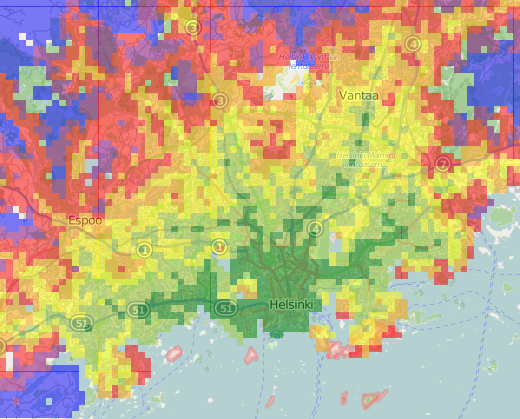
\includegraphics[width=8cm]{images/isarithmic-example.png}
    \caption{An approximated isarithmic map depicting travel times to Helsinki center.}
    \label{fig:isarithmicimpl}
  \end{center}
\end{figure}

\subsection{Dot Maps and Proportional Symbol Maps}

The application supports producing dot and proportional symbol maps by providing the Dot mapping module. With default configuration, the module produces dot maps, but it is possible to provide an option for calculating and using proportional symbol values. For enabling the user to get more information about data points, it is possible to provide the user information bubbles which are activated by clicking the symbol. The module also supports using customized symbols for data points, the default being a simple Leaflet marker.

\subsection{Input Formats}

All implemented mapping modules use GeoJSON as their input format. GeoJSON is the \emph{de facto} format for transmitting geographical data on the web \citep{bostock_code_2013}. There is also great support for GeoJSON data in the existing software, for example in the Leaflet map library used by the application. However, due to its verboseness, GeoJSON may be unsuitable for simpler data sets and visualizations such as dot maps. Therefore, we have specified and implemented support for converters for transforming data to GeoJSON format. Currently, only converting ``flat dot'' (see appendix \ref{appendix:flatdotformat}) format is supported. An example of the format converter functionality is presented in listing \ref{listing:inputformats}.

\begin{lstlisting}[caption=An example code for using the flat dot input format converter.,language=JavaScript,label=listing:inputformats]
var data = fetch('markers.json')
  .then(function(resp) { return resp.json(); })
  .then(thematic.converters.flatToGeoJSON);
module.setData(data);
\end{lstlisting}

Typically, the data is fetched from an external resource (external API or a separate JSON file) asynchronously. Therefore, the modules support using ECMAScript Promises\footnote{\url{https://developer.mozilla.org/en/docs/Web/JavaScript/Reference/Global_Objects/Promise}} to pass visualized data. However, also synchronous data (such as using data defined in the source code file) is supported by wrapping the values in Promise objects.

\subsection{Value Normalization}

When visualizing a metric such as average temperature of an area, the scale of values is completely different from when visualizing, say, population density. Therefore, in order to provide general-purpose map visualization tools, it is necessary to support displaying a wide variety of values and scales.

For this application, we decided to implement a highly versatile normalization functionality which allows the visualizer to work on virtually any scale. Instead of transforming the input values into a predefined value set, the application transforms the input values directly to a visualizable value, such as ``red'' on a choropleth map, or ``10px'' on a proportional symbol map. Moreover, this mechanism is compatible with, e.g., scaling functionality of D3.js\footnote{\url{http://d3js.org/}, \url{https://github.com/mbostock/d3/wiki/Scales}} visualization library, so the visualizer can leverage the sophisticated scaling functionality of external libraries. An example of a Thematic.js scale functionality is presented in listing \ref{listing:valuenormalization}

\begin{lstlisting}[caption=An example of Thematic.js scale functionality.,language=JavaScript,label=listing:valuenormalization]
// a standalone scale function
var scale = function(value) {
  var colors = [
    {time: 30, color: 'green'},
    {time: 40, color: 'yellowgreen'},
    {time: 50, color: 'yellow'},
    {time: 60, color: 'orange'},
    {time: 80, color: 'red'},
    {time: 100, color: 'purple'},
    {time: 120, color: 'blue'}
  ];

  return _.find(colors, 
    color => value <= color.time) || _.last(colors);
}

module.setScale(scale);

// a scale function using the d3.js library
var d3scale = d3.scale.linear()
  .domain([60, 65, 70])
  .range(['#e5f5f9', '#99d8c9', '#2ca25f']);

module2.setScale(d3scale):
\end{lstlisting}

\subsection{Modularity and Extendability}

It is hardly possible to cover the whole area of geographic visualizations. Therefore, instead of trying to support every visualization method possible, we implemented the architecture of the application so that it is as straightforward as possible to extend the functionality.

As a result of this, visualization methods can be easily extended by adding tailored mapping modules to the application. Additionally, it is possible to create customized aggregators, converters and scales and bundle these as an extension to the application.

~

\fixme{Would the implementation chapter need more practical examples, be it code or screenshots?}
